%%%% fatec-article.tex, 2024/03/10

\documentclass[
  a4paper,%% Tamanho de papel: a4paper, letterpaper (^), etc.
  12pt,%% Tamanho de fonte: 10pt (^), 11pt, 12pt, etc.
  english,%% Idioma secundário (penúltimo) (>)
  brazilian,%% Idioma primário (último) (>)
]{article}

%% Pacotes utilizados
\usepackage[]{fatec-article}
\usepackage{float}
\usepackage{setspace}
\usepackage{graphicx}
\usepackage{pdfpages}

%% Início do documento
\begin{document}
\vspace{8cm}
\begin{center}
    \large \textbf{\title{ARTEFATOS DO PROJETO DE SOFTWARE}}
\end{center}

\maketitle

\break

\tableofcontents

\break


%exemplo da forma de organização das seções e subseções, você deverá adaptar o template para a realidade do seu projeto.

\section*{Diário de Bordo}
\addcontentsline{toc}{section}{Diário de Bordo}

O Diário de Bordo tem como objetivo facilitar a organização do andamento do projeto, por meio dos registros das atividades e tarefas.
    
    Na Figura \Cref{fig:dia} é possível ver como foi feita a distribuição das atividades do projeto:

    \begin{figure}[H]
        \centering
        \caption{Diário de Bordo}
        \label{fig:dia}
        
\includegraphics[width=\textwidth,page=1]{Logos/fatec-template.pdf}
        
\includepdf[pages=2-]{Logos/fatec-template.pdf}
        \SourceOrNote{Autoria própria (2024)}
    \end{figure}

\section*{Diagramas UML}
    Nesta seção serão apresentados os diagramas da UML utilizados para a modelagem do sistema desenvolvido. Dentre os diagramas utilizados, pode-se citar: Diagrama de Caso de Uso, Diagrama de Classe e Diagrama de Objetos.
    
    \subsection*{Diagrama de Caso de Uso}
    \addcontentsline{toc}{section}{Diagrama de Caso de Uso}

    A seguir na \Cref{fig:diagrama-caso-uso}, os atores do sistema e suas devidas funções dentro do sistema:

\begin{enumerate}
    \item Proxy/Squid: atua como intermediador das solicitações realizadas dos usuários à Internet, o qual efetua o gerenciamento dos sites bloqueados ou não, além do registro de informações de acesso. 
    \item Administrador: possui privilégios  para gerenciar o sistema, as permissões de acesso de outros usuários, os bloqueios de forma manual, e sites que são exceção, obtém as estatísticas de bloqueios e seu histórico.
    \item Aluno: este não ira interagir diretamente com o sistema, mas apenas visualizar a tela de bloqueio caso o site seja bloqueado.
    
\end{enumerate}

\begin{figure}[H]
    \centering
    \caption{Diagrama de caso de uso}
    \label{fig:diagrama-caso-uso}
    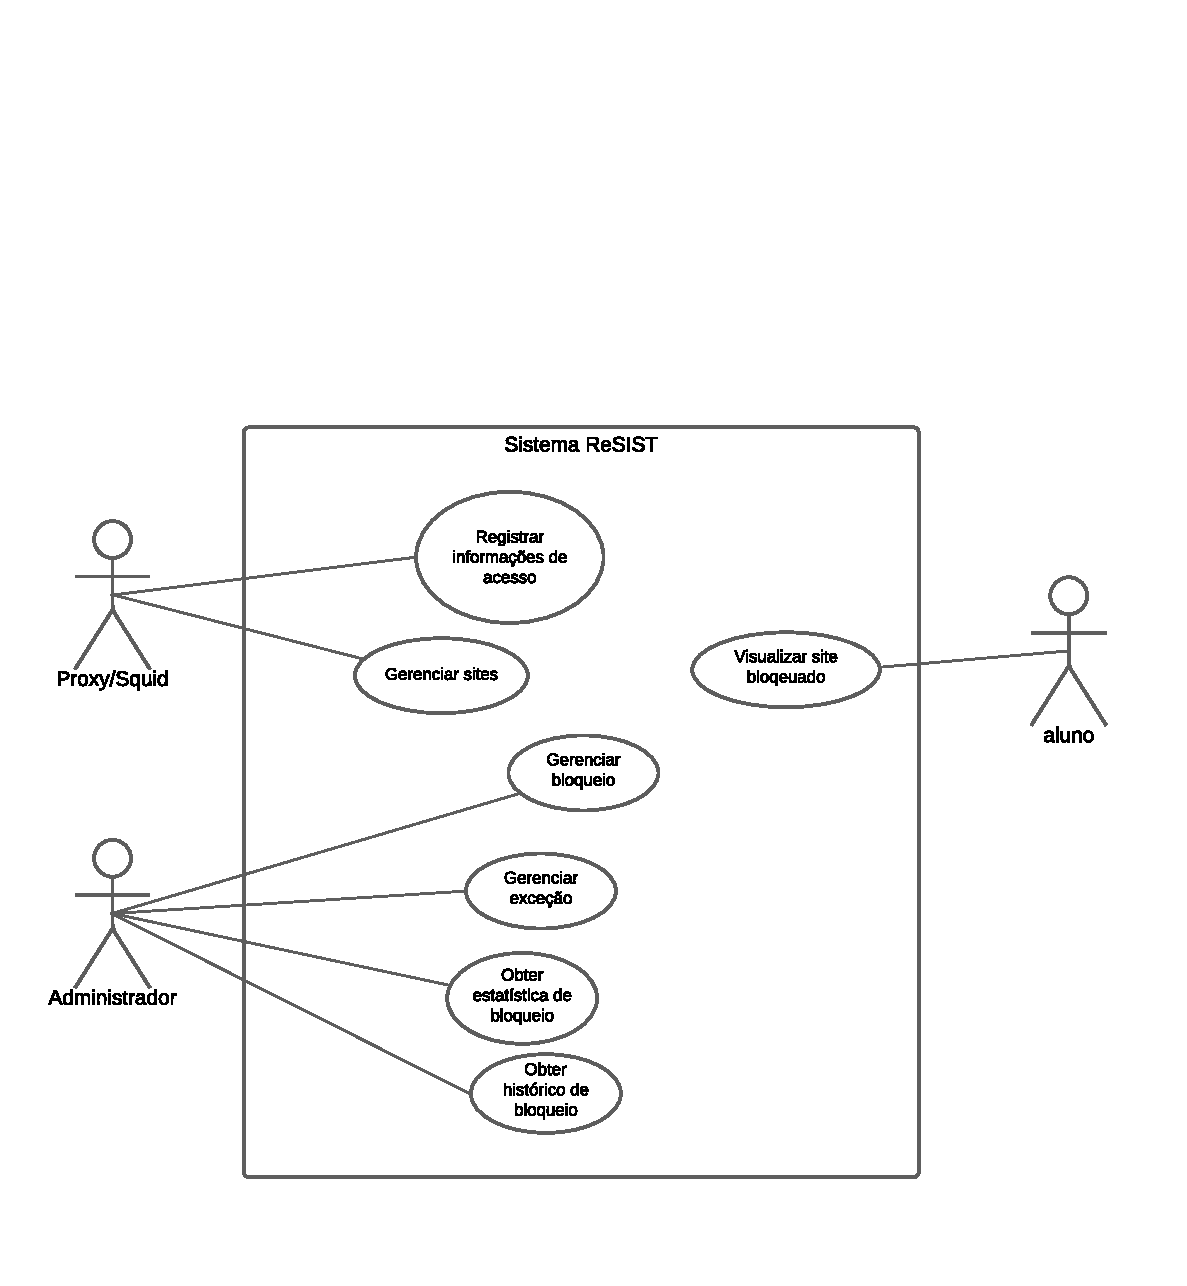
\includegraphics[width=\textwidth]{Logos/UML-Casos-de-uso.pdf}
    \SourceOrNote{Autoria prória  (2024)}
\end{figure}

    
    
    \subsection*{Diagrama de Classe}
    \addcontentsline{toc}{section}{Diagrama de Classe}

    Esse é um exemplo de diagrama de classe, você deverá descrever os elementos presentes no diagrama (classes e relacionamentos).

    \begin{figure}[H]
        \centering
        \caption{Diagrama de caso de uso}
        \label{fig:diagrama-caso-uso}
        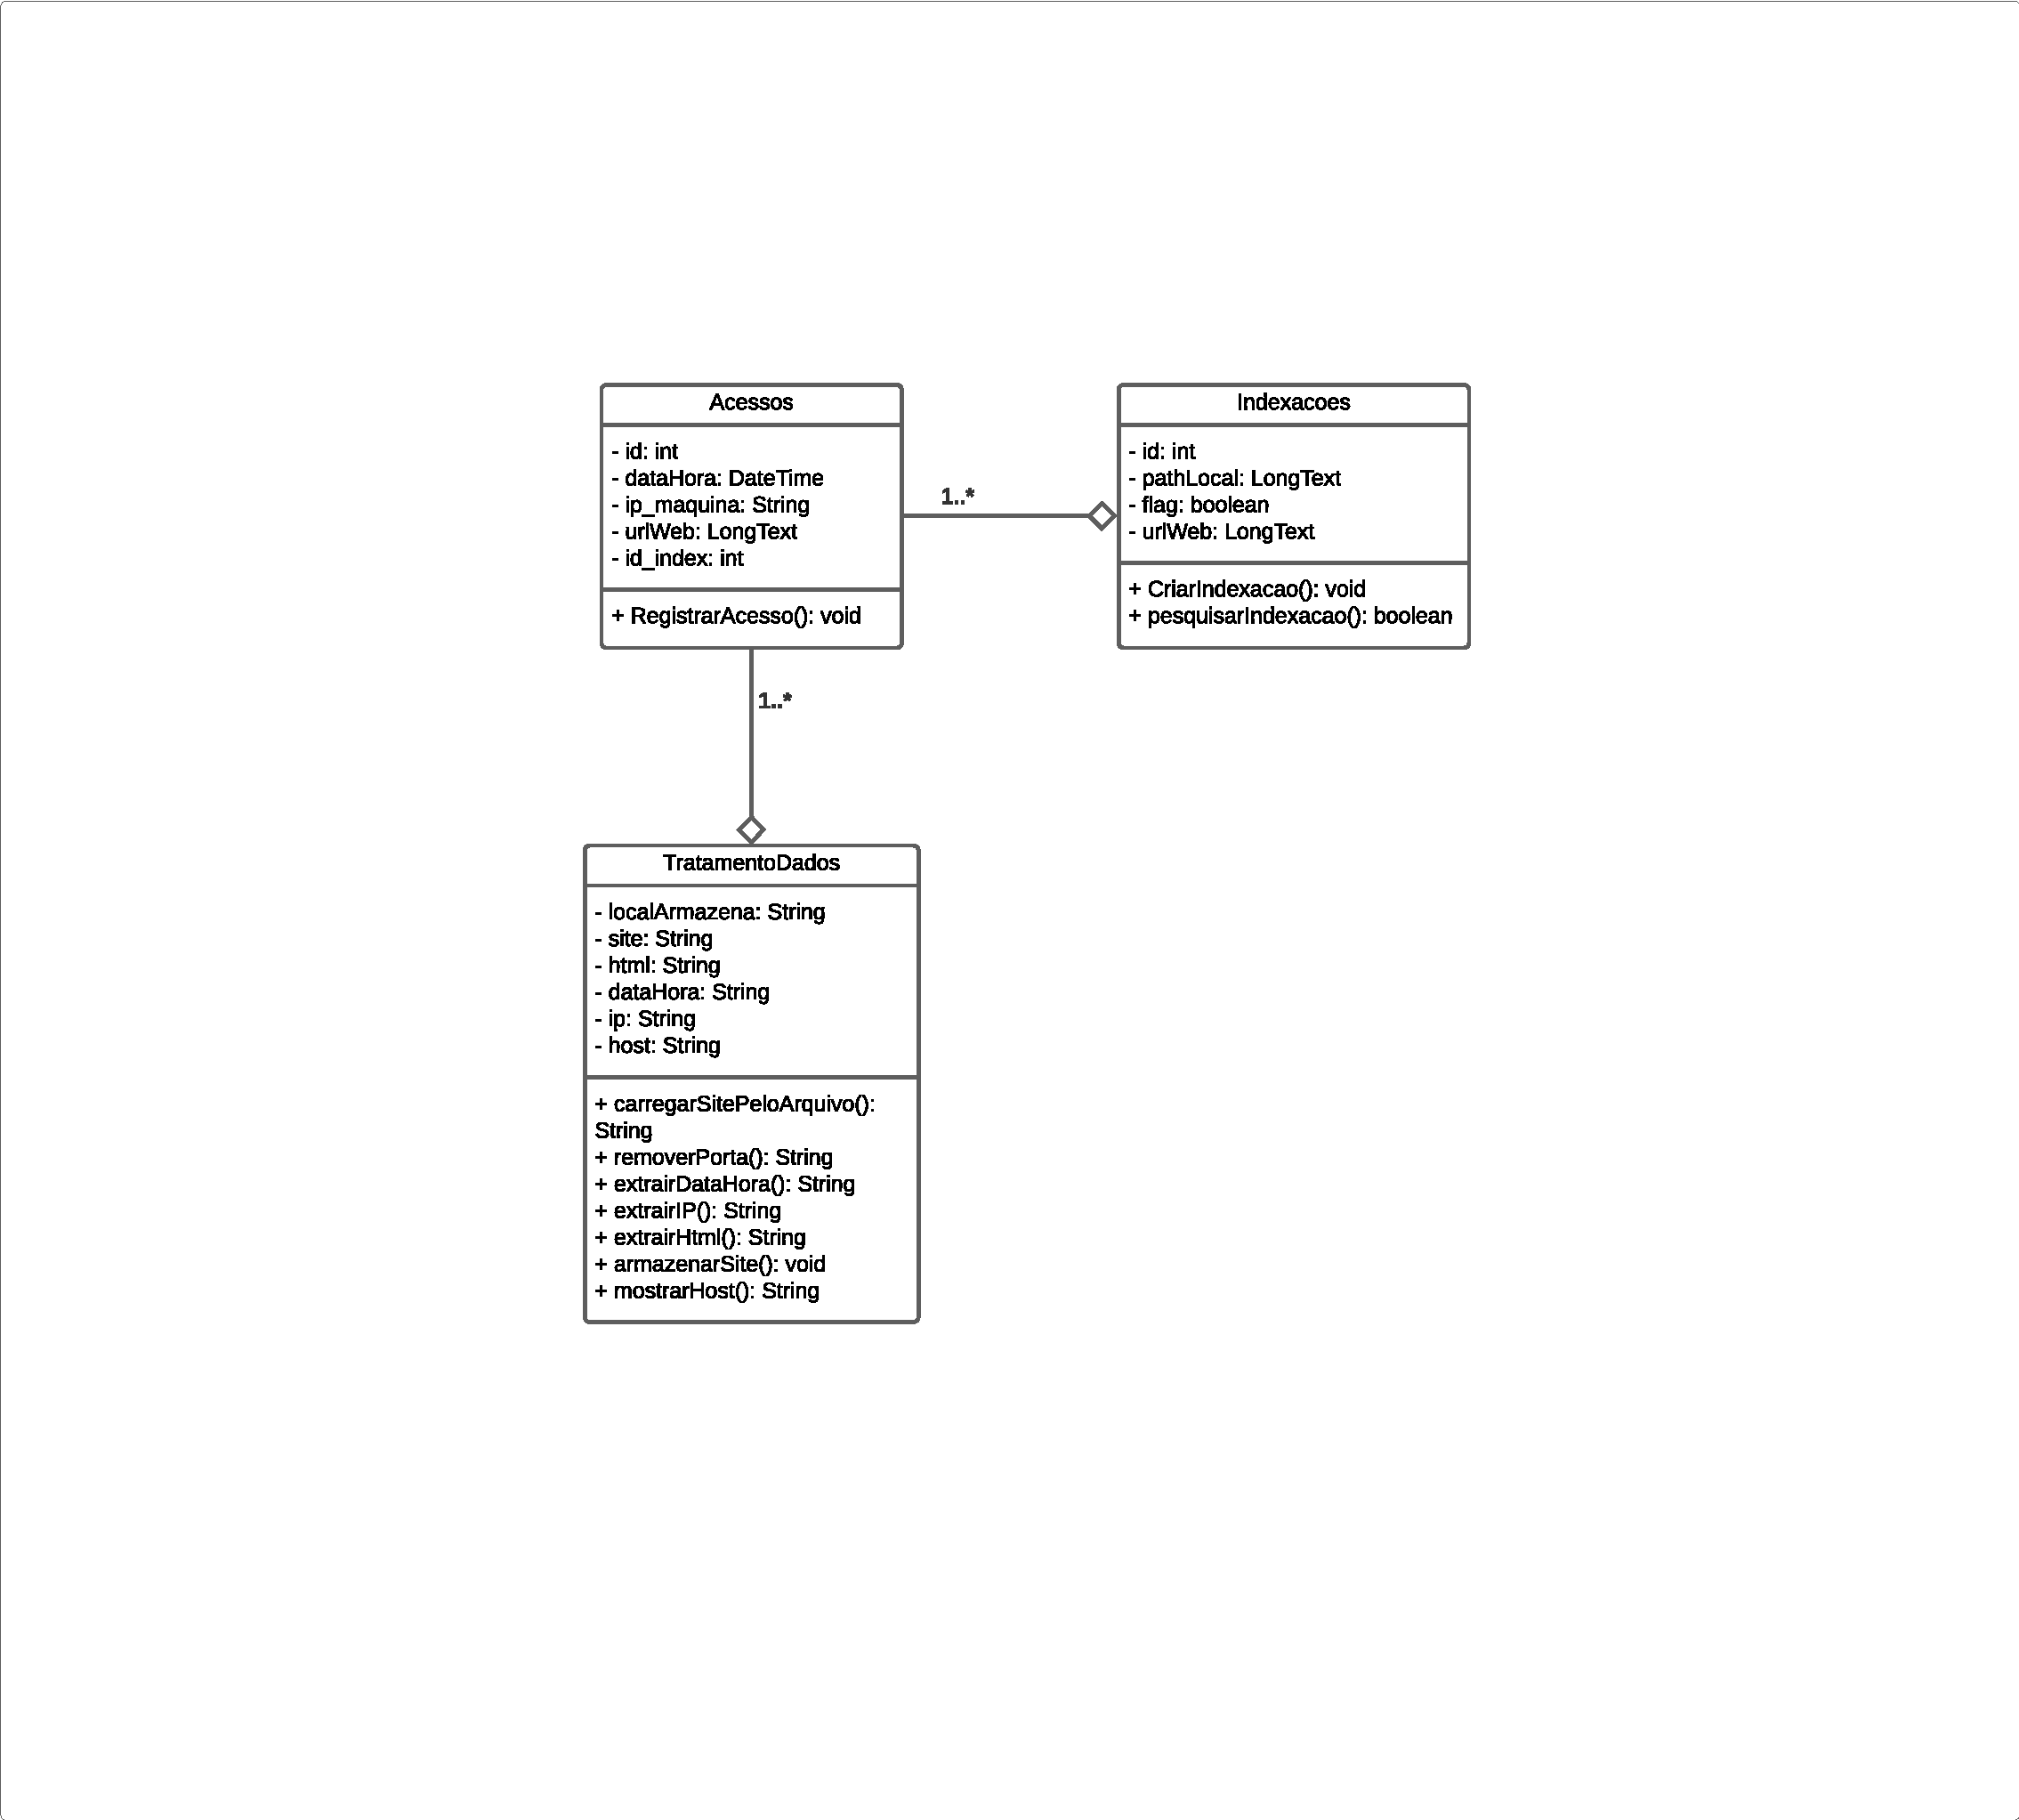
\includegraphics[width=\textwidth]{Logos/diagrama-de-Classes.pdf}
        \SourceOrNote{Autoria prória  (2024)}
    \end{figure}

     

    \subsection*{Diagrama de Objetos}
    \addcontentsline{toc}{section}{Diagrama de Objetos}


\begin{figure}[H]
    \centering
    \caption{Diagrama de caso de uso}
    \label{fig:diagrama-caso-uso}
    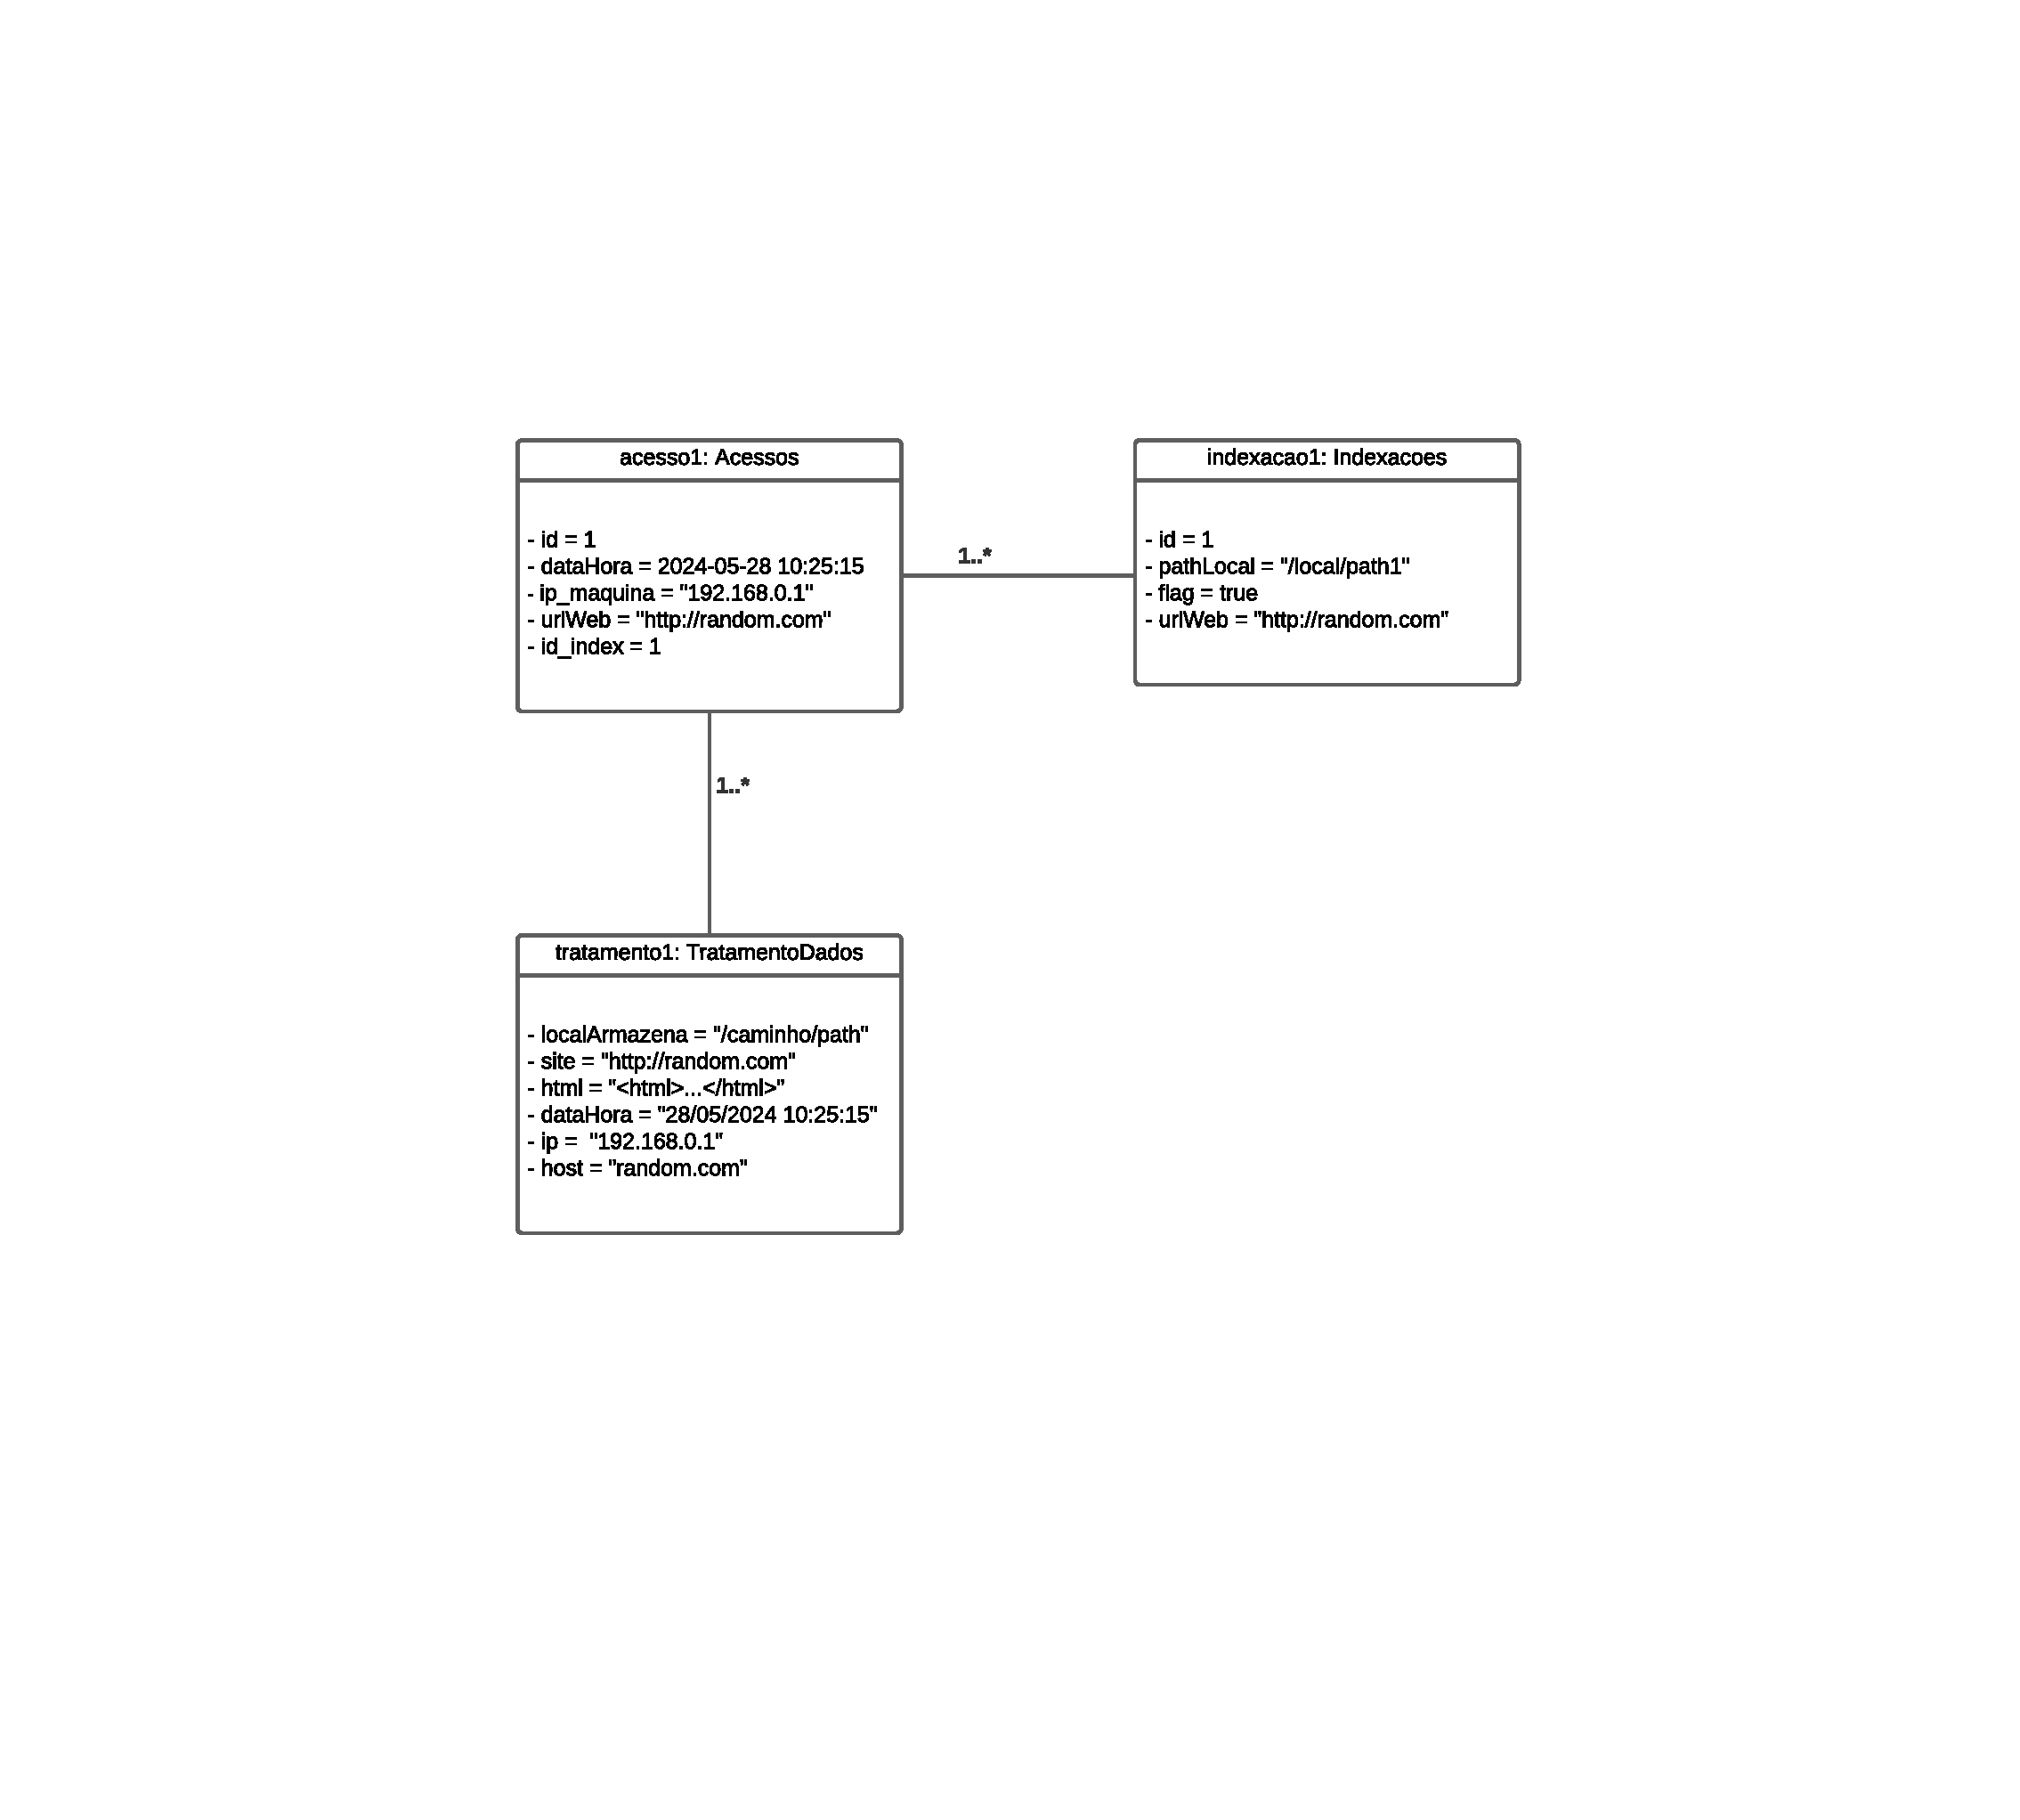
\includegraphics[width=\textwidth]{Logos/diagrama-de-Objetos.pdf}
    \SourceOrNote{Autoria prória  (2024)}
\end{figure}

Por meio destes diagramas é possível visualizar de maneira simplória as principais funcionalidades do sistema.

\section*{Diagramas de Entidades e Relacionamentos}

O DER (Diagrama de Entidade-Relacionamento), é uma maneira de representar de forma visual e detelhada as entidades, atributos e conexões do banco de dados
\subsection*{Diagrama do Modelo Conceitual}
    \addcontentsline{toc}{section}{Diagrama do Modelo Conceitual}
    O banco de dados está dividido em duas partes principais, do sistema sendo a principal: 
    acessos, responsável por guardar os dados necessários para geração de relatórios, quando o estudante acessar um site, será extraído as seguintes informações: data e hora, o ip da máquina que foi acessada e a url do site. Indexações: foi criado com pensando na IA, o pathLocal, armazena o caminho para um arquivo txt, o qual contém o conteúdo do site em HTML, assim a Inteligência Artificíal poderá realizar a analise à procura por um termo de injuria racial.
    
    A flag, vai ser o meio para identificar se o site está bloqueado ou não. Em urlWeb,  como o próprio nome diz, é gravado a url do site.
    
    A segunda parte é a do usuário, engloba informações da instiruição, pessoais e as permissões que o usuário possui dentro do sistema.


    \begin{figure}[H]
        \centering
        \caption{Diagrama do Modelo Conceitual}
        \label{fig:conceit}
        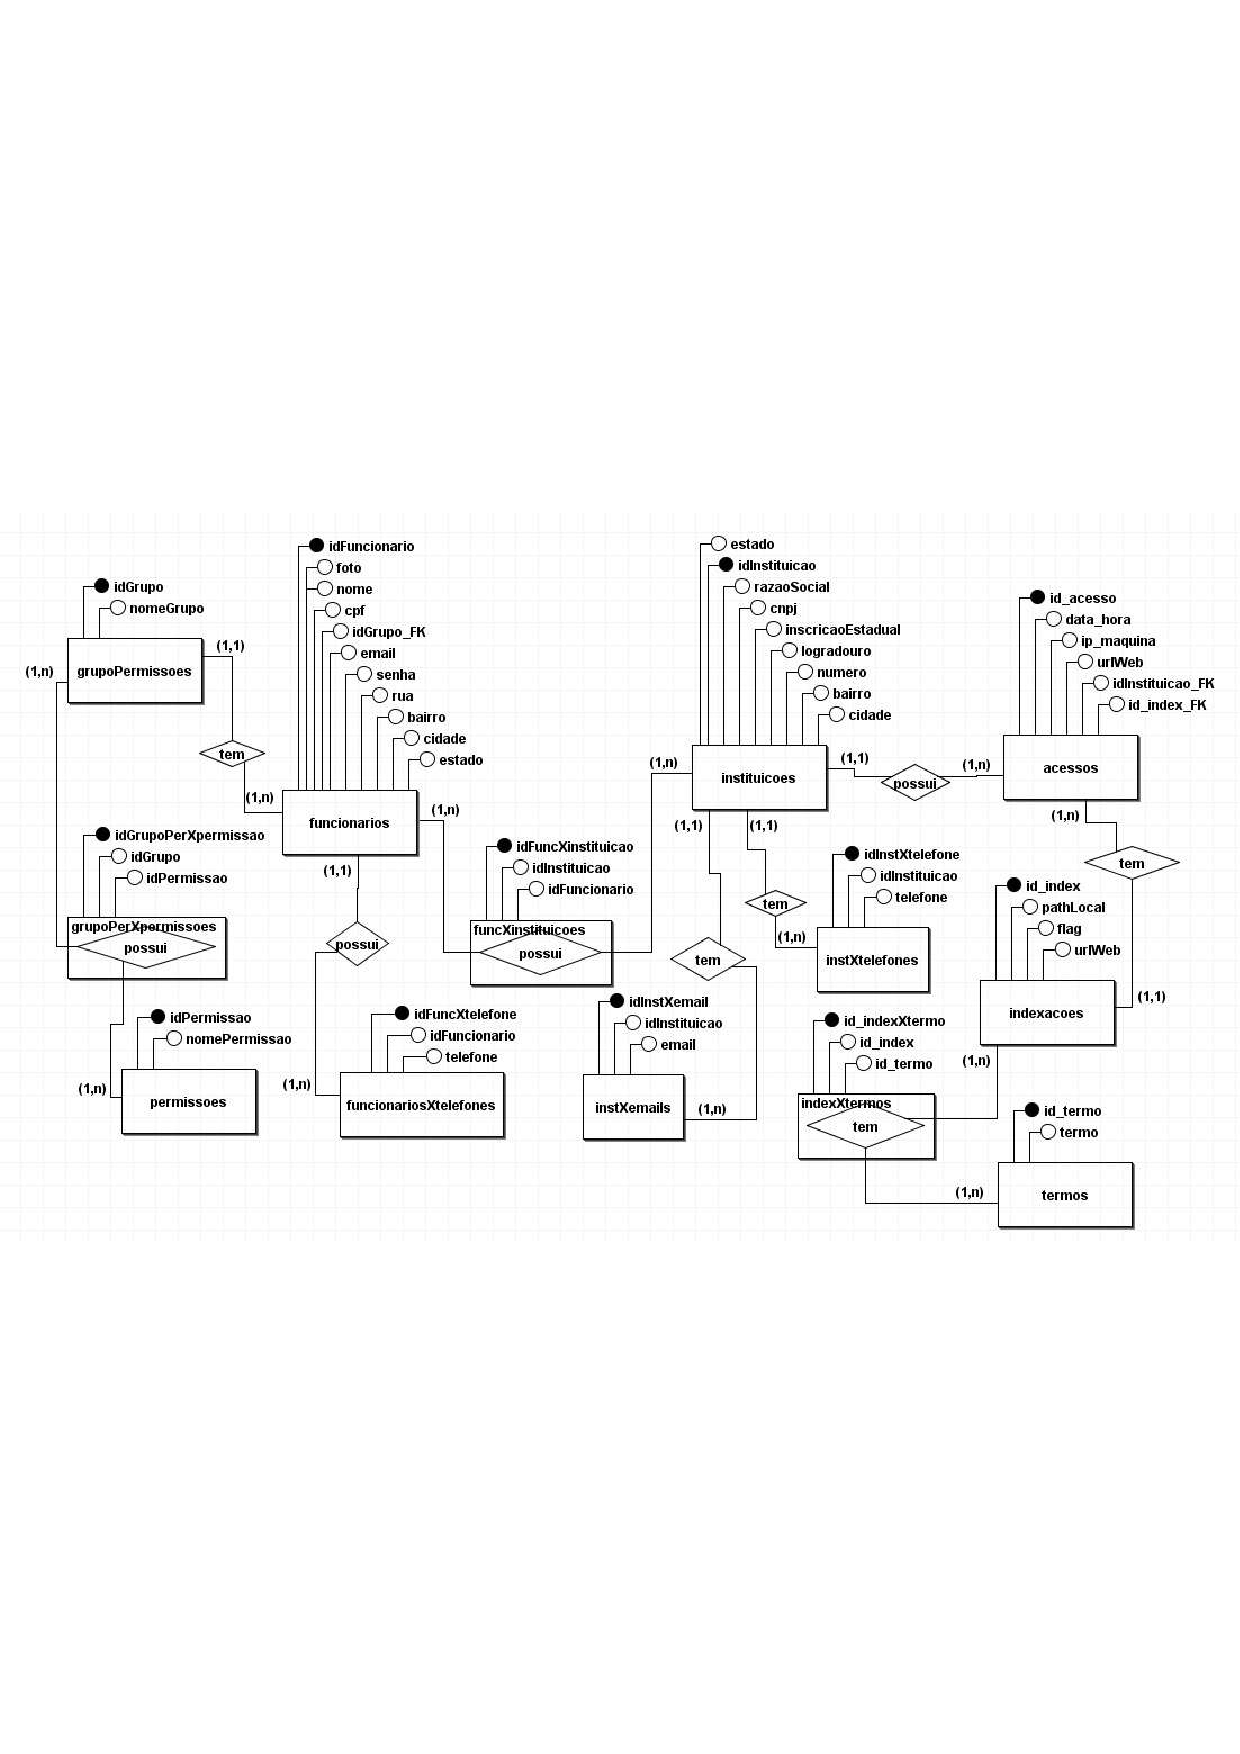
\includegraphics[width=\textwidth]{Logos/Conceitual-ReSist-PDF.pdf}
        \SourceOrNote{Autoria prória  (2024)}
    \end{figure}
    O banco de dados está dividido em duas partes principais, do sistema sendo a principal: 
    acessos, responsável por guardar os dados necessários para geração de relatórios, quando o estudante acessar um site, será extraído as seguintes informações: data e hora, o ip da máquina que foi acessada e a url do site. Indexações: foi criado com pensando na IA, o pathLocal, armazena o caminho para um arquivo txt, o qual contém o conteúdo do site em HTML, assim a Inteligência Artificíal poderá realizar a analise à procura por um termo de injuria racial.
    
    A flag, vai ser o meio para identificar se o site está bloqueado ou não. Em urlWeb,  como o próprio nome diz, é gravado a url do site.
    
    A segunda parte é a do usuário, engloba informações da instiruição, pessoais e as permissões que o usuário possui dentro do sistema.


    \begin{figure}[H]
        \centering
        \caption{Diagrama do Modelo lógico}
        \label{fig:log}
        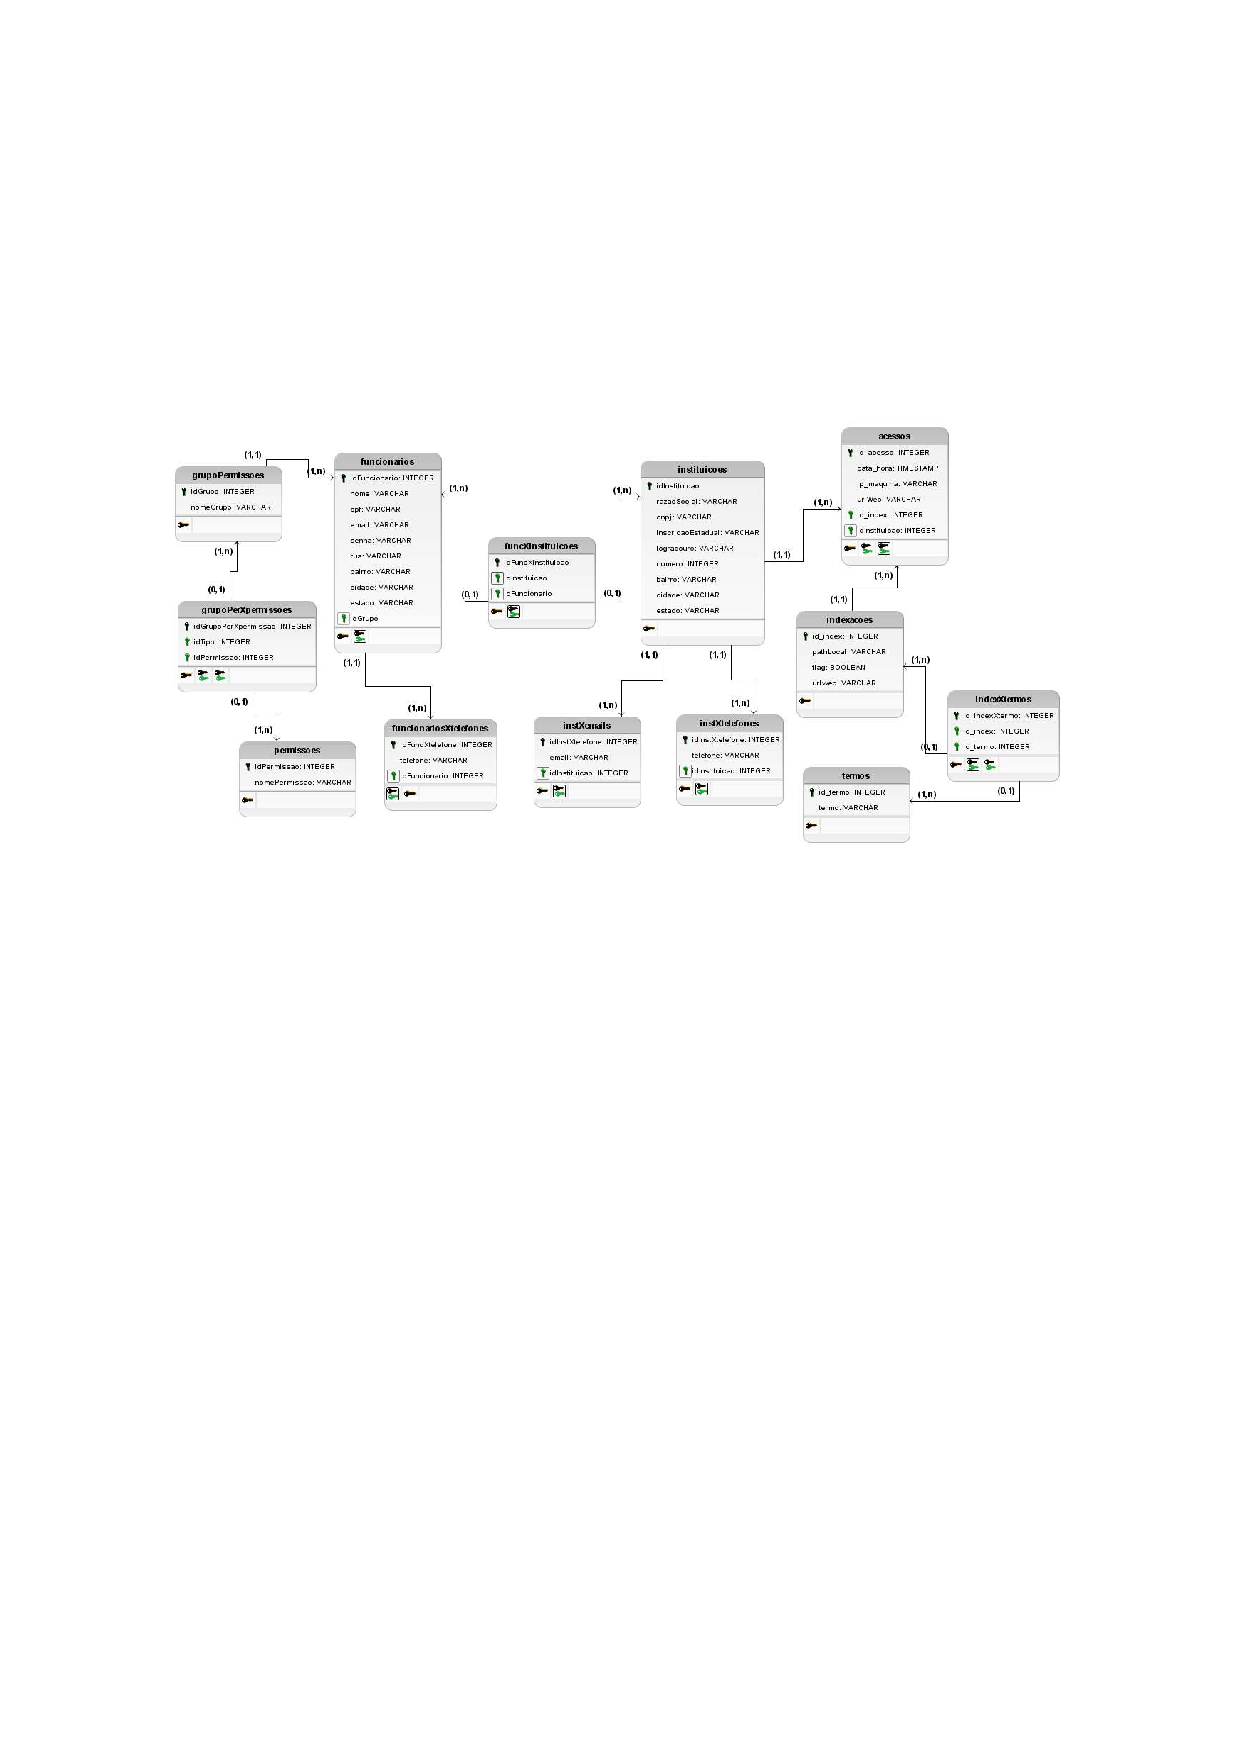
\includegraphics[width=\textwidth]{Logos/Logico-ReSist-PDF.pdf}
        \SourceOrNote{Autoria prória  (2024)}
    \end{figure}

    A  \Cref{fig:log}, representa o diagrama do modelo lógico do sistema. A diferença significativa deste para o conceitual, é a inclusão dos tipos de dados dos atributos, encarregados por definir o formato dos dados registrados das colunas da tabela. 

    % \begin{figure}[H]
    %     \centering
    %     \caption{Diagrama do Modelo Físico}
    %     \label{fig:log}
    %     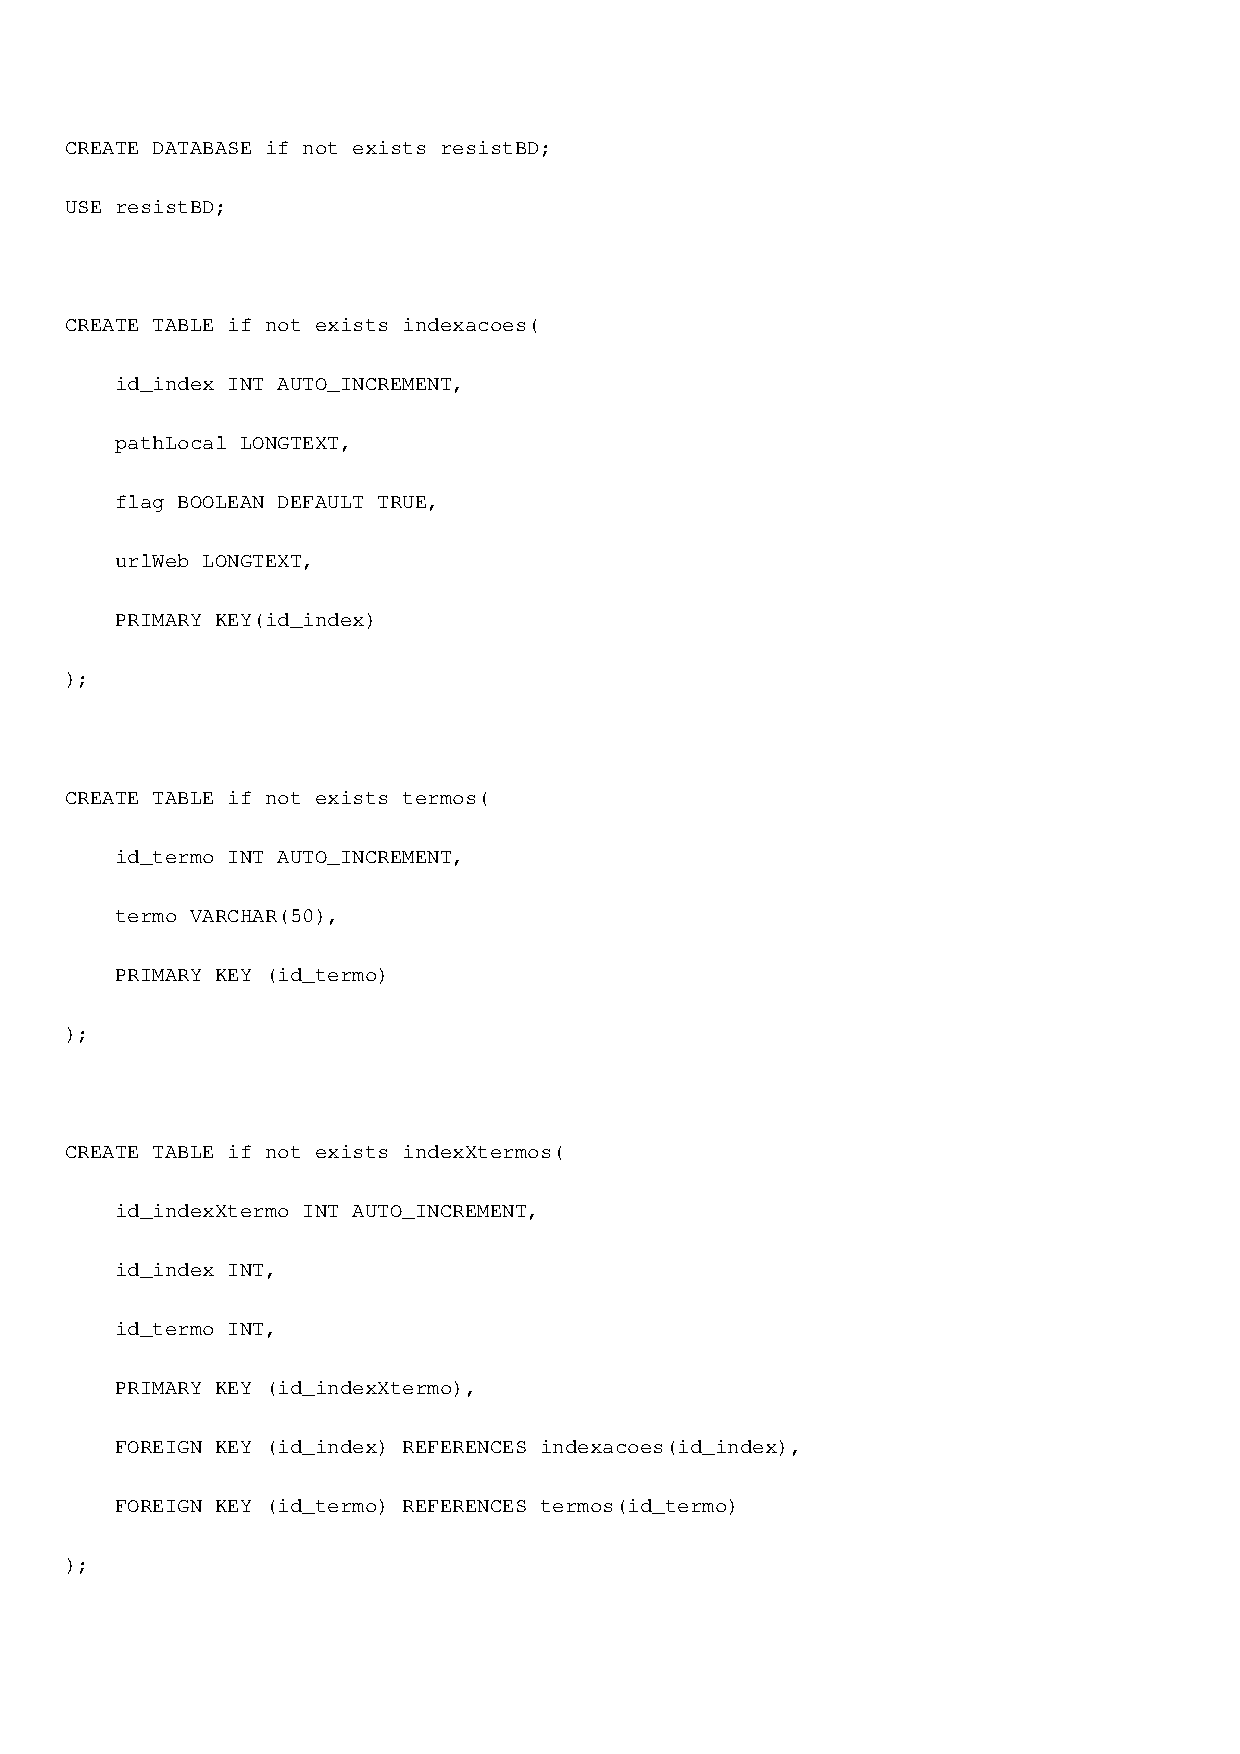
\includegraphics[width=\textwidth]{Logos/resistBD_script.pdf}
    %     \SourceOrNote{Autoria prória (2024)}
    % \end{figure}

    % Força nova página
\clearpage

% Primeira página como figura
\begin{figure}[H]
    \centering
    \caption{Diagrama do Modelo Físico}
    \label{fig:fis}
    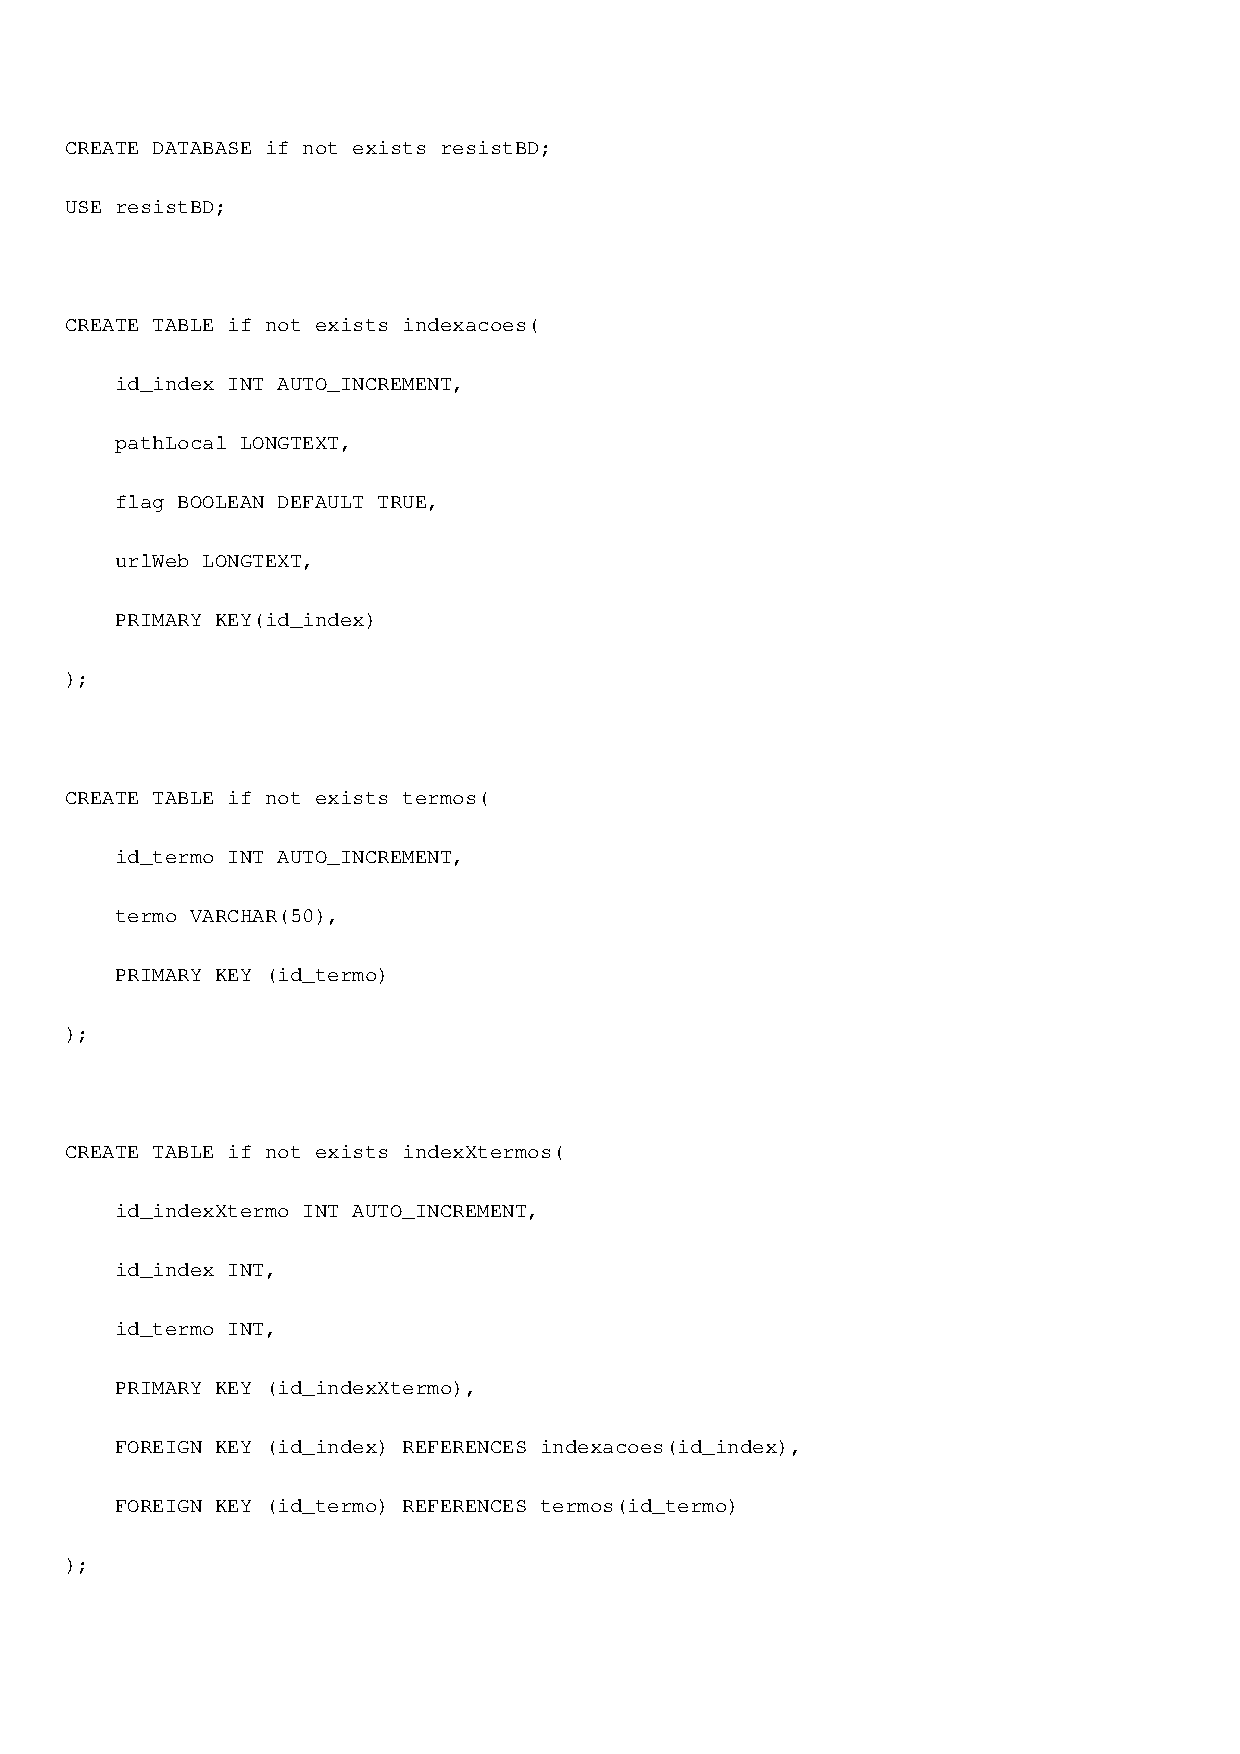
\includegraphics[width=\textwidth,page=1]{Logos/resistBD_script.pdf}
\end{figure}

% Páginas restantes
\includepdf[pages=2-]{Logos/resistBD_script.pdf}

% Adiciona a fonte após o PDF
\begin{center}
    \SourceOrNote{Autoria própria (2024)}
\end{center}

% Força próxima seção em nova página
\clearpage

    O modelo físico garante maior eficiência no processamento de consultas e transações, ao alinhar a estrutura do banco às necessidades específicas da aplicação, minimizando redundâncias e maximizando a velocidade de acesso aos dados.
    \section*{Canvas}
    \addcontentsline{toc}{section}{Canvas}
    O modelo de negócio Canvas na \Cref{fig:can}, visa criar o sistema ReSist, com o uso da Inteligência Artificial(IA) para detectar e auxiliar no combate à discriminação online em ambientes educacionais.

    A proposta valor é centrada na identificação com precisão de injúria racial em textos diversos, o qual proporciona um ambiente mais inclusivo e seguro para a educação. A plataforma será divulgada por meio de website, redes sociais, email, marketing e telefone. \newline O relacionamento com os clientes ira ser preservado através de suporte técnico, treinamento na utilização do sistema, e feedback.

    As atividades-chaves incluem desenvolver o sistema, o monitoramento do banco de dados, treinamento do sistema, marketing e vendas. Os recursos-chaves são a equipe de desenvolvimento e analistas de dados, algoritmos de IA e infraestrutura robusta de TI. 

    Parcerias serão estabelecidas com instituições de ensino, desenvolvedores de software e especialistas em direitos humanos e a dicriminação.

    A estrutura de custos envolve desenvolvimento do sistema, custos operacionais, marketing e vendas, enquanto a receita será gerada por meio de assinaturas mensais ou anuais pagas pelas instituições de ensino e outras organizações que utilizarem a plataforma.


    \begin{figure}[H]
        \centering
        \caption{Canvas}
        \label{fig:can}
        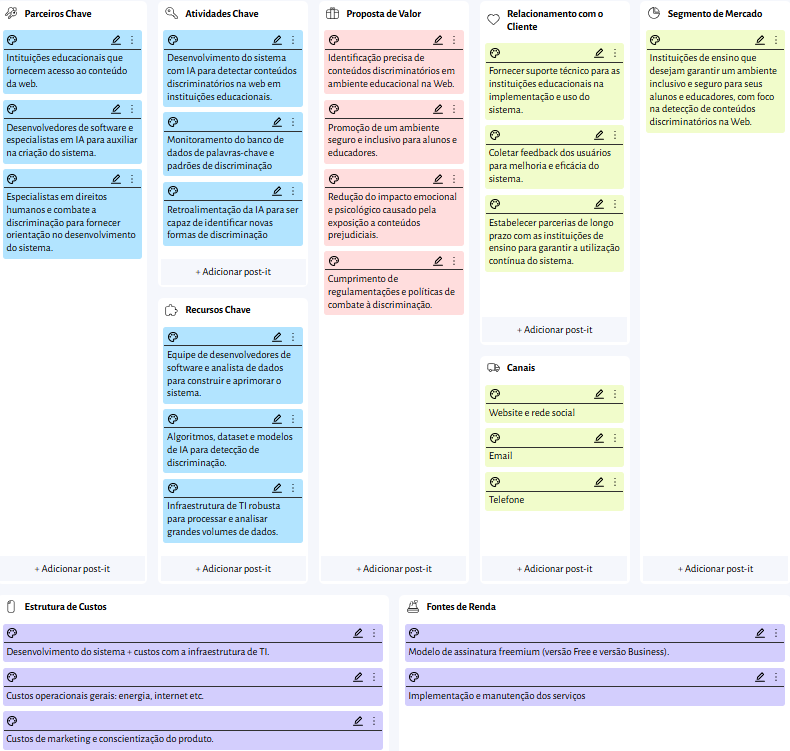
\includegraphics[width=\textwidth]{Logos/canvas.png}
        \SourceOrNote{Autoria prória (2024)}
    \end{figure}


    \section*{Diagrama de redes}
    \addcontentsline{toc}{section}{Diagrama de redes}

    O diagrama de rede \Cref{fig:red} é composto por um esquema que inclui uma rede interna, Firewall (IA), um servidor proxy (squid), um modem (roteador), e a rede externa (internet). A rede interna é formada por máquinas (computadores)utilizadas por usuários (discentes e/ ou docentes), sendo assim, para a rede interna  realizar a sua comunicação com a rede externa (internet), ela deve passar por outros processos que irão proteger os dados dos usuários e manter outros quesitos de segurança para os mesmos. 

O firewall é a etapa do diagrama de redes responsável por filtrar conteúdos indesejados, também sendo capaz de bloquear ataques direcionados a rede interna. O servidor é responsável por estabelecer a comunicação segura e mascarar o IP interno, para o acesso com a rede externa; além disso, o Proxy é utilizado para armazenar os acessos e informações gerais do usuário na rede externa. O moden, também conhecido por Roteador, tem como serventia a passagem da internet, estabelecer sua conexão, como se fosse o “Porto” da internet.

Por fim a rede externa, também conhecida como internet, é a ferramenta aonde usuários tem a possibilidade de se conectar e estabelecer uma comunicação de forma remota com outro usuário.

Sendo assim, o diagrama de redes traça um caminho de como seria a comunicação entre a rede interna com a rede externa, passando por todos os processos necessários para essa conexão.

\begin{figure}[H]
    \centering
    \caption{Diagrama de redes}
    \label{fig:red}
    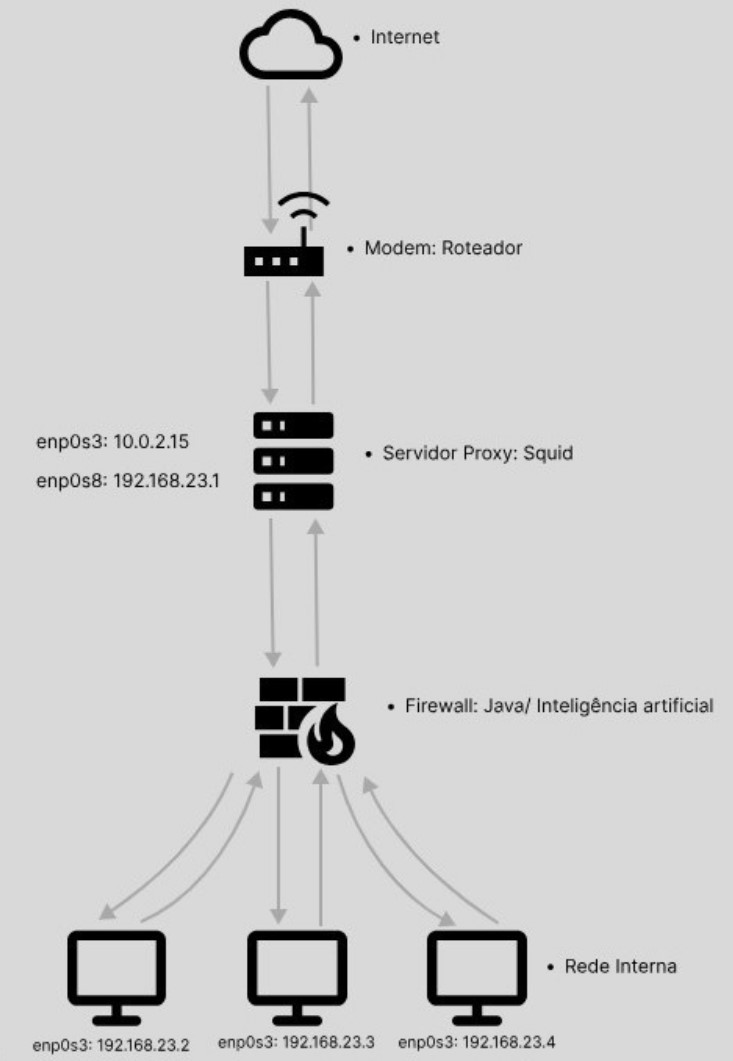
\includegraphics[width=0.4\textwidth]{Logos/JPG-diagrama-de-redes.jpg}
    \SourceOrNote{Autoria prória (2024)}
\end{figure}

\section*{UI de Alta Fidelidade}
\addcontentsline{toc}{section}{UI de Alta Fidelidade}
   
    
    \subsection*{Dashboard}
    \addcontentsline{toc}{section}{Dashboard}
    A \Cref{fig:dashboard}, ilustra a tela inicial, tratando-se de um \textit{Dashboard} que proporciona um resumo das informações coletadas, como a atividade recente, que apresenta todas as atualizações do ambiente; visão geral dos bloqueios, trazendo a quantidade de bloqueios e a evolução em relação ao mês anterior; nível de incidência por laboratório (no exemplo, tratam-se de laboratórios de informática em um ambiente escolar); histórico por data, e os laboratórios que estão ativos no momento.

    \begin{figure}[H]
        \centering
        \caption{Dashboard}%
        \label{fig:dashboard}
        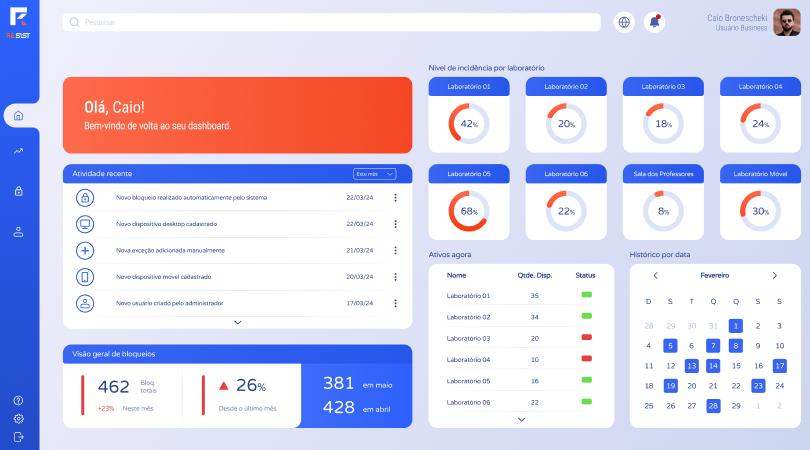
\includegraphics[scale=.7]{tdashboard}
        \SourceOrNote{Autoria Própria (2024)}
        \end{figure}

        \subsection*{Estatísticas}
        \addcontentsline{toc}{section}{Estatísticas}

        A \Cref{fig:estatistica} exibe a aba de estatísticas, onde há uma visualização aprofundada dos dados de bloqueio, exibindo a quantidade de bloqueios em dispositivos móveis e \textit{Desktop}, uma comparação do aumento ou diminuição mês-a-mês, e alguns dos últimos bloqueios, realizando a distinção entre os automáticos e manuais.

        \begin{figure}[H]
            \centering
            \caption{Estatísticas}%
            \label{fig:estatistica}
            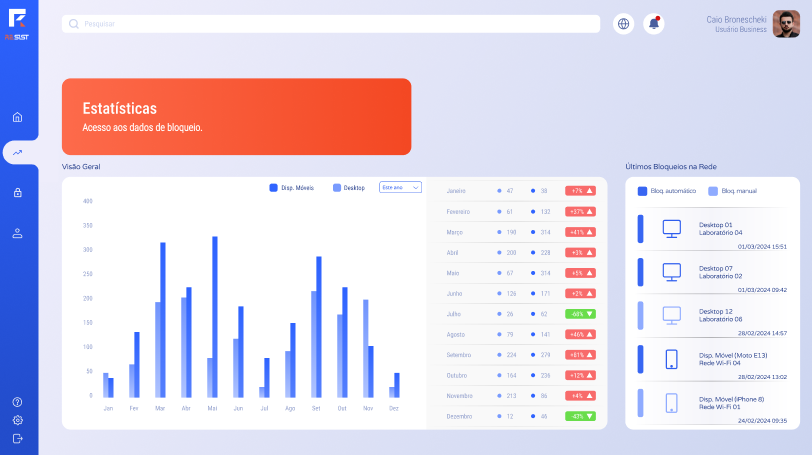
\includegraphics[scale=.7]{testatistica}
            \SourceOrNote{Autoria Própria (2024)}
            \end{figure}


        \subsection*{Bloqueios}
        \addcontentsline{toc}{section}{Bloqueios}

        A página bloqueios \Cref{fig:Bloqueios}, representada na figura 3, exibe uma visão aprofundada sobre cada bloqueio realizado. É exibida uma tabela com a URL bloqueada, a data do bloqueio e se foi manual ou automático. A página disponibiliza ainda uma funcionalidade para bloquear um \textit{Website} manualmente, especificando o motivo e período do bloqueio. É possível editar os bloqueios já realizados, para caso seja necessário cancelá-los.
        
        \begin{figure}[H]
            \centering
            \caption{Bloqueios}%
            \label{fig:Bloqueios}
            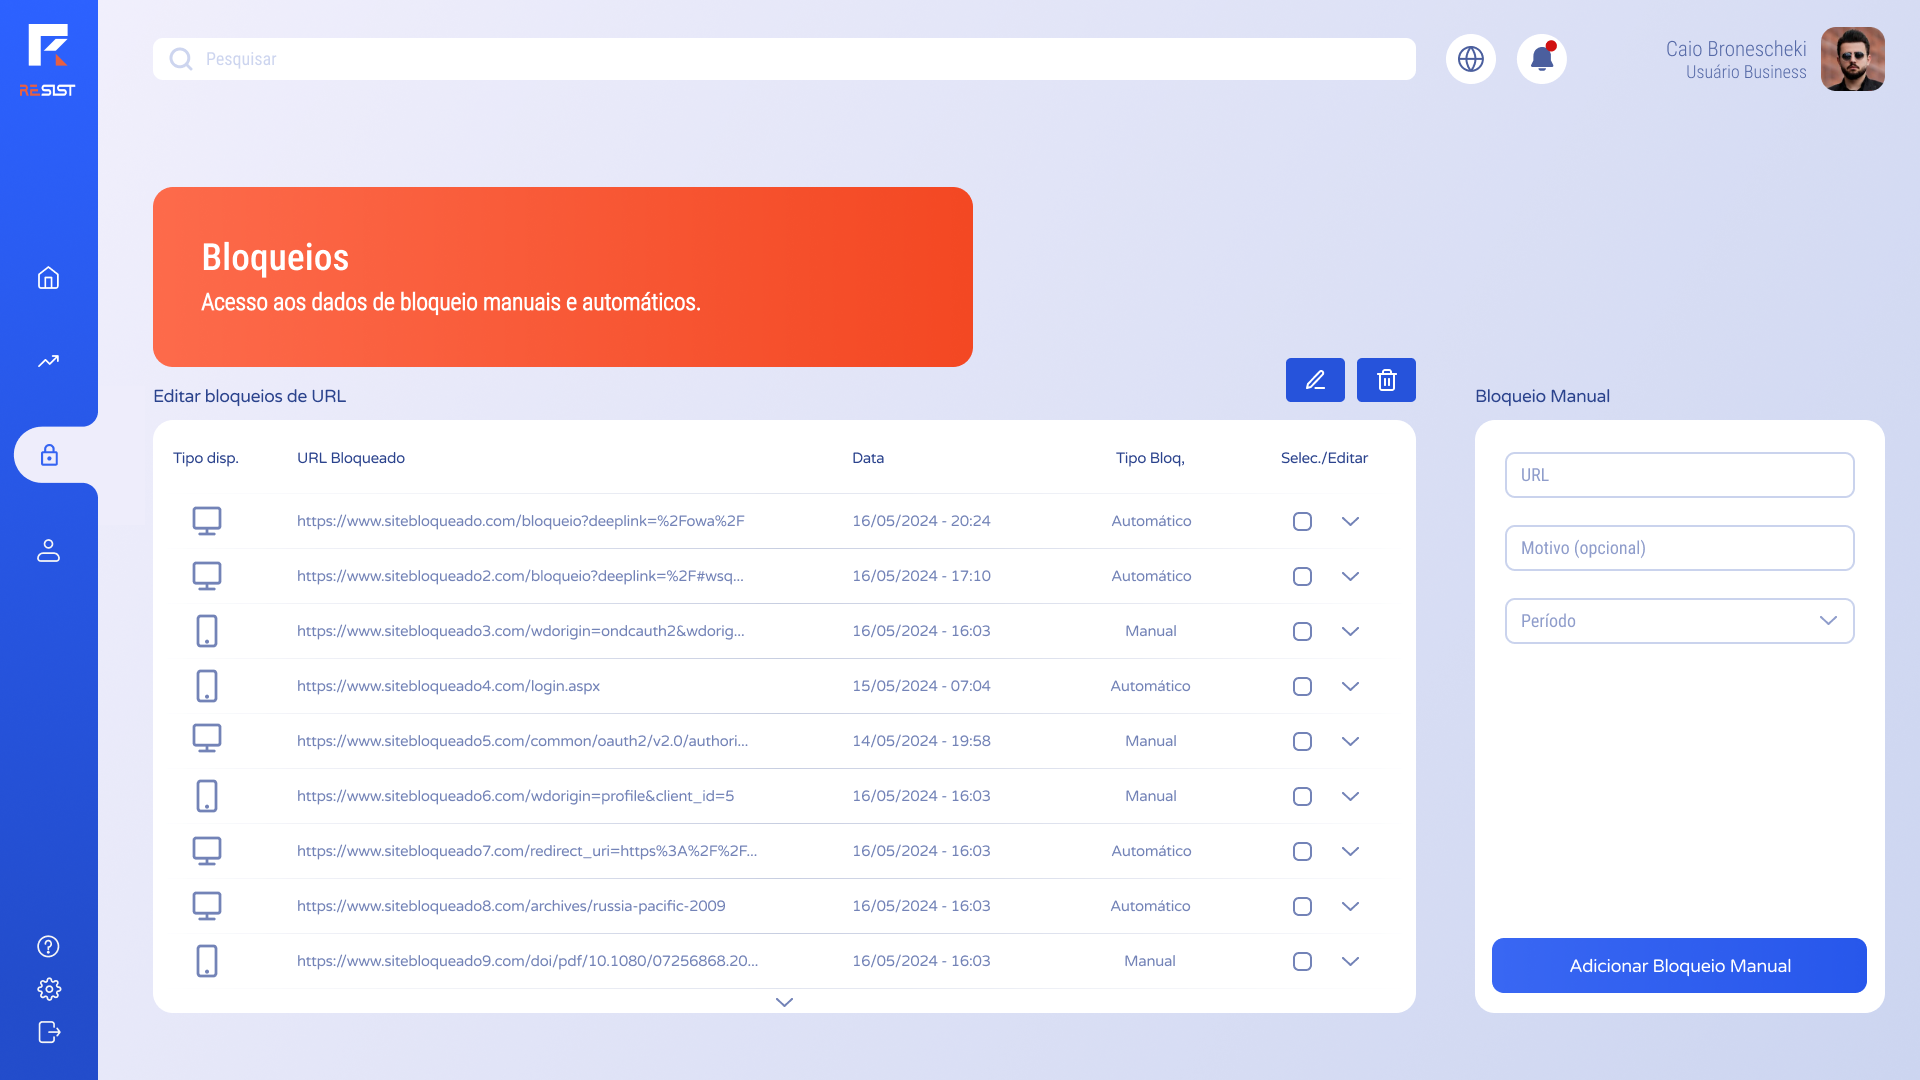
\includegraphics[scale=.19]{bloqueios}
            \SourceOrNote{Autoria Própria (2024)}
            \end{figure}

            \subsection*{Usuários}
            \addcontentsline{toc}{section}{Usuários}
            
            
            Na \Cref{fig:usu}, a página de gerenciamento dos usuários exibe todos os perfis cadastrados no ambiente, com nome completo, cargos de cada um, email e disponibilidade. Além das opções de cadastrar e alterar informações dos usuários.
            \begin{figure}[H]
                \centering
                \caption{Usuários}%
                \label{fig:usu}
                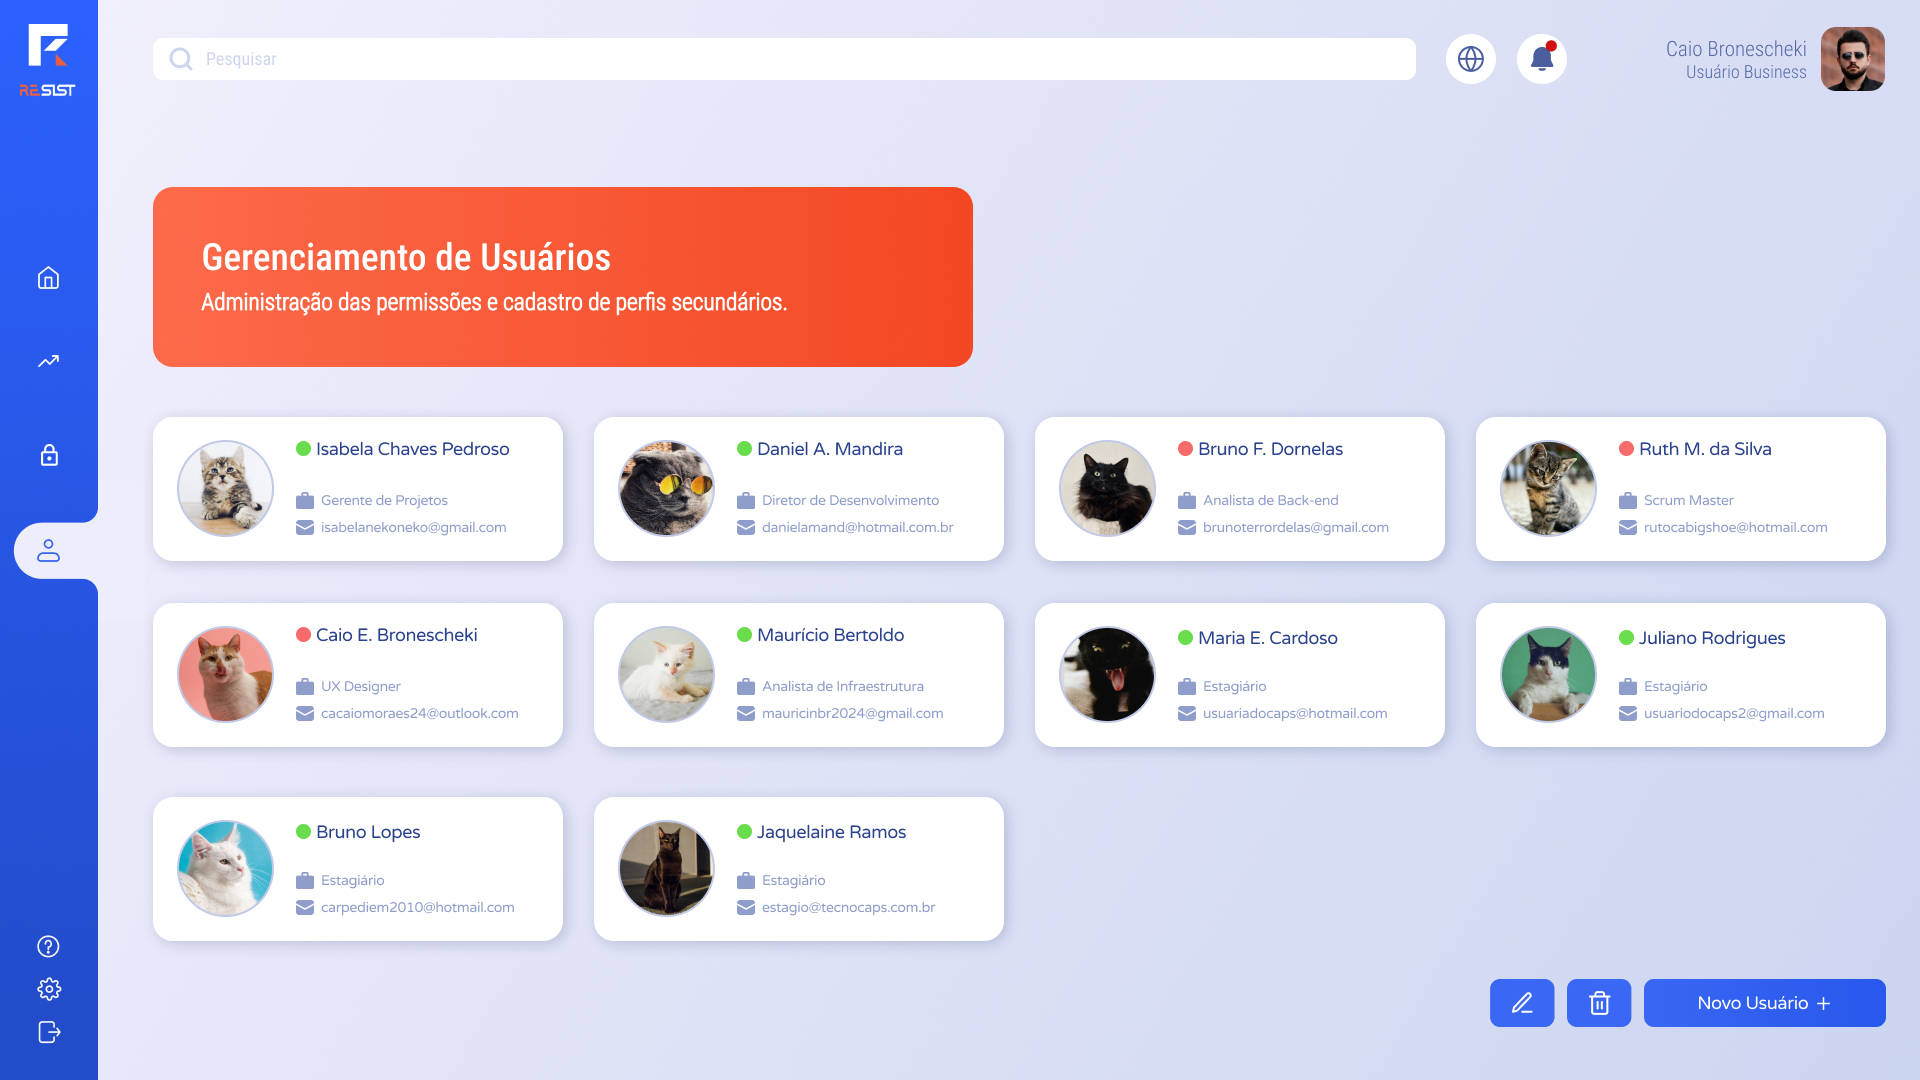
\includegraphics[scale=.19]{tusuario}
                \SourceOrNote{Autoria Própria (2024)}
                \end{figure}

            
            Portanto, por meio da exibição dos dados coletados, pode se proporcionar uma visão clara dos elementos centrais do sistema e uma compreensão visual fiel da funcionalidade e interatividade presente no sistema, a fim de reforçar seu papel como uma ferramenta para a identificação e combate a discriminação em ambientes educacionais, tanto no ambiente Web, como fora. Vale ressaltar que todas as telas foram criadas com o intuito de concentrar os mínimos detalhes de forma concisa para que o usuário possa ter acesso as informações necessárias de forma concentrada, 
            
            
            
            
\section*{Scrum e Kanban}
\addcontentsline{toc}{section}{Scrum e Kanban}

O Scrum é um framework ágil focado na gestão eficiente de projetos, especialmente no desenvolvimento de software. Ele organiza o trabalho em ciclos curtos chamados sprints, que variam de 2 a 4 semanas, onde a equipe entrega incrementos do produto de forma contínua. A flexibilidade do Scrum permite que a equipe se adapte rapidamente a mudanças, com foco em iterações rápidas, comunicação constante e envolvimento direto do cliente, garantindo que as soluções atendam às necessidades reais do projeto. O Scrum enfatiza a autogestão da equipe e a transparência do processo, o que facilita a identificação e correção de problemas rapidamente. A seguir três fases do kanban durante uma semana: Na \Cref{fig:1}, há quatro tarefas para começar; já na \Cref{fig:2}, a tarefa "Banner" está em progresso; na \Cref{fig:3} já não há mais tarefas para serem iniciadas, todas foram finalizadas apenas "LaTex - artigo" esta em progresso. 

\begin{figure}[H]
    \centering
    \caption{1º visão}%
    \label{fig:1}
    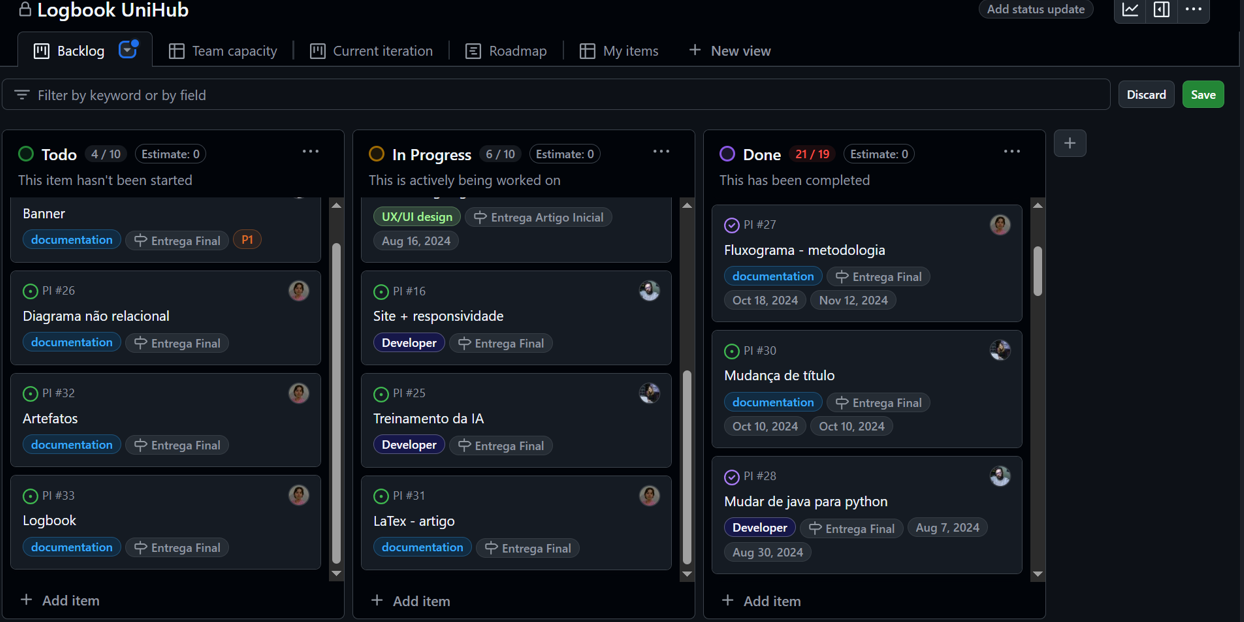
\includegraphics[scale=.38]{kan1}
    \SourceOrNote{Autoria Própria (2024)}
    \end{figure}


    \begin{figure}[H]
        \centering
        \caption{2º visão}%
        \label{fig:2}
        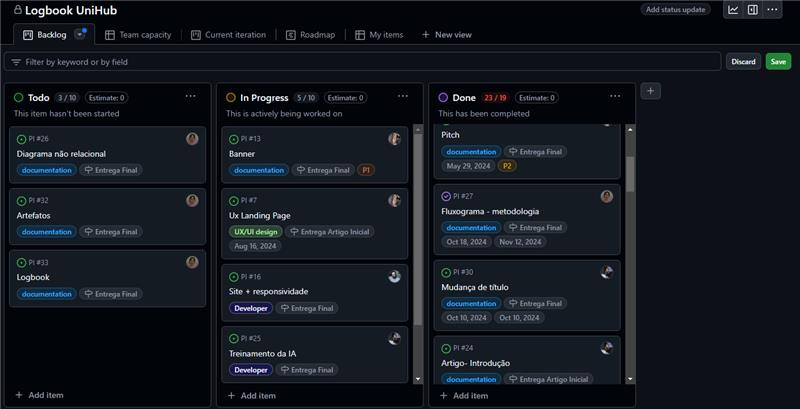
\includegraphics[scale=.6]{kan2}
        \SourceOrNote{Autoria Própria (2024)}
        \end{figure}


        \begin{figure}[H]
            \centering
            \caption{3º visão}%
            \label{fig:3}
            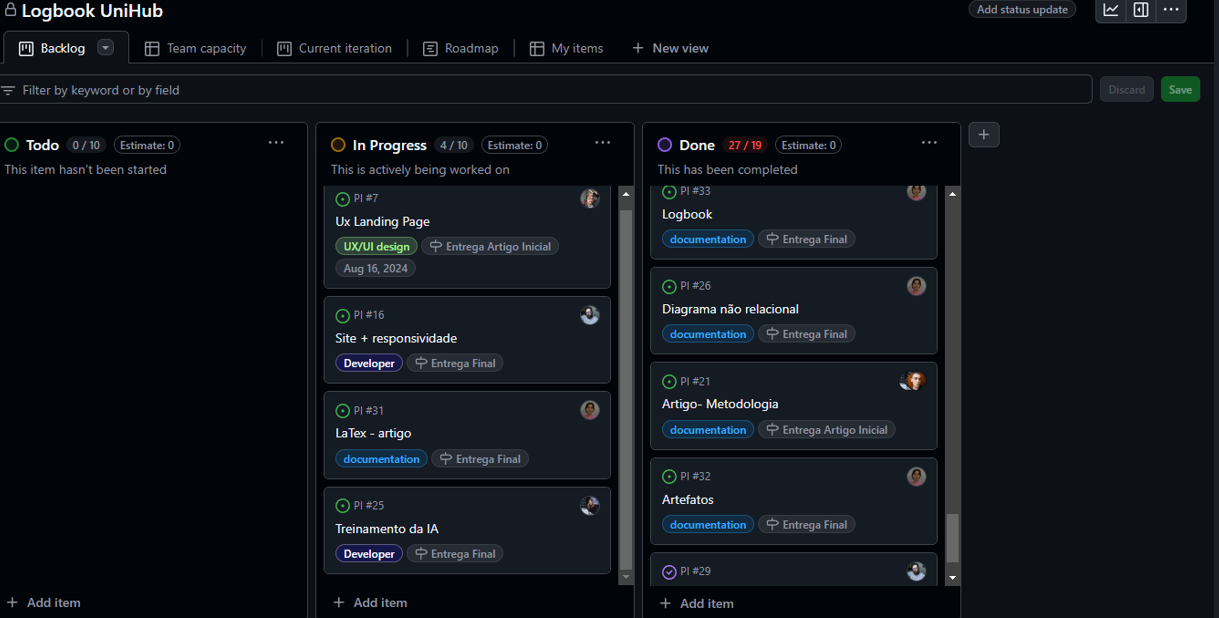
\includegraphics[scale=.38]{kan3}
            \SourceOrNote{Autoria Própria (2024)}
            \end{figure}











        
    




\end{document}
